%!TEX root = 2015-07.tex
\section{Pixelweise-Klassifikation}

\subsection*{Pixelweise-Klassifikation}

\begin{frame}{Bildweise Klassifikation}

\begin{minipage}{0.49\textwidth}
\begin{center}
ImageNET
\end{center}
\vspace{1cm}
\end{minipage}
\begin{minipage}{0.49\textwidth}
\begin{center}
MNIST
\end{center}
\vspace{1cm}
\end{minipage}

\end{frame}


\begin{frame}{Problemstellung \& Anwendungen}

\begin{minipage}{0.49\textwidth}
\begin{center}
Autonomes Fahren
\end{center}
\vspace{1cm}
\end{minipage}
\begin{minipage}{0.49\textwidth}
\begin{center}
Medizininformatik
\end{center}
\vspace{1cm}
\end{minipage}

\begin{center}
Bildbearbeitung
\end{center}



\end{frame}

\begin{frame}[squeeze]{Sliding-Window Ansatz}
\vspace{-1em}
\begin{figure}[H]
	\centering
	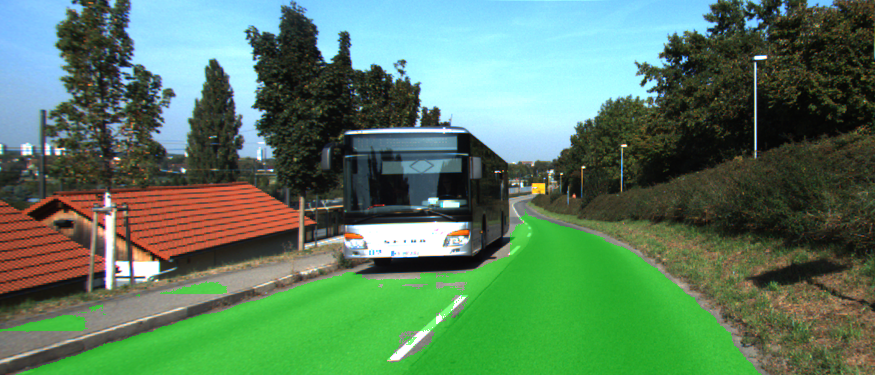
\includegraphics[width=0.8\textwidth]{../images/street.png}
	%\caption{Visualization of the classification problem solved by our neural network.}
	%\label{fig:figure}
\end{figure}
\vspace{-.2em}
\begin{minipage}{0.6\textwidth}
\centering
\fbox{
	\begin{tabular}{l l}
		\multicolumn{2}{l}{\textbf{Klassifikation Netz}} \\
		\textit{Input:} & Ein $n \times n$ Pixel \\
						& großer Bildauschnitt. \\
		\textit{Output:} & 1, falls der center Pixel \\
		                 &  Straße ist.\\
	\end{tabular}
}
\end{minipage}
\begin{minipage}{0.39\textwidth}
\begin{figure}[H]
	\centering
	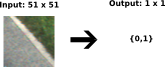
\includegraphics[width=\textwidth]{../images/sliding_window.png}
	%\caption{Visualization of the classification problem solved by our neural network.}
	%\label{fig:figure}
\end{figure}
\end{minipage}


\end{frame}

\begin{frame}{Sliding-Window im Netz}

\end{frame}

\begin{frame}{Deconvolution Netzwerke}

\begin{minipage}[b]{0.49\textwidth}
\begin{figure}[H]
	\centering
	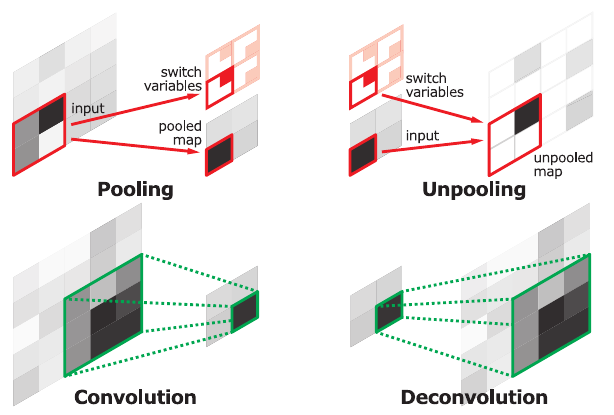
\includegraphics[width=0.8\textwidth]{../images/deconv.png}
	\caption*{\scriptsize{Funktionsweise eines Deconvolution Layers}}
\end{figure}
\end{minipage}
\begin{minipage}[b]{0.49\textwidth}
\begin{figure}[H]
	\centering
	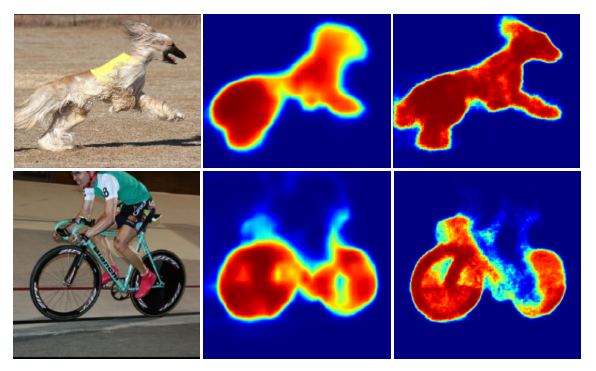
\includegraphics[width=0.8\textwidth]{../images/heatmap.png}
	\caption*{\scriptsize{Heatmap erzeugt durch Deconvolution Netz}}
\end{figure}
\end{minipage}

\begin{figure}[H]
	\centering
	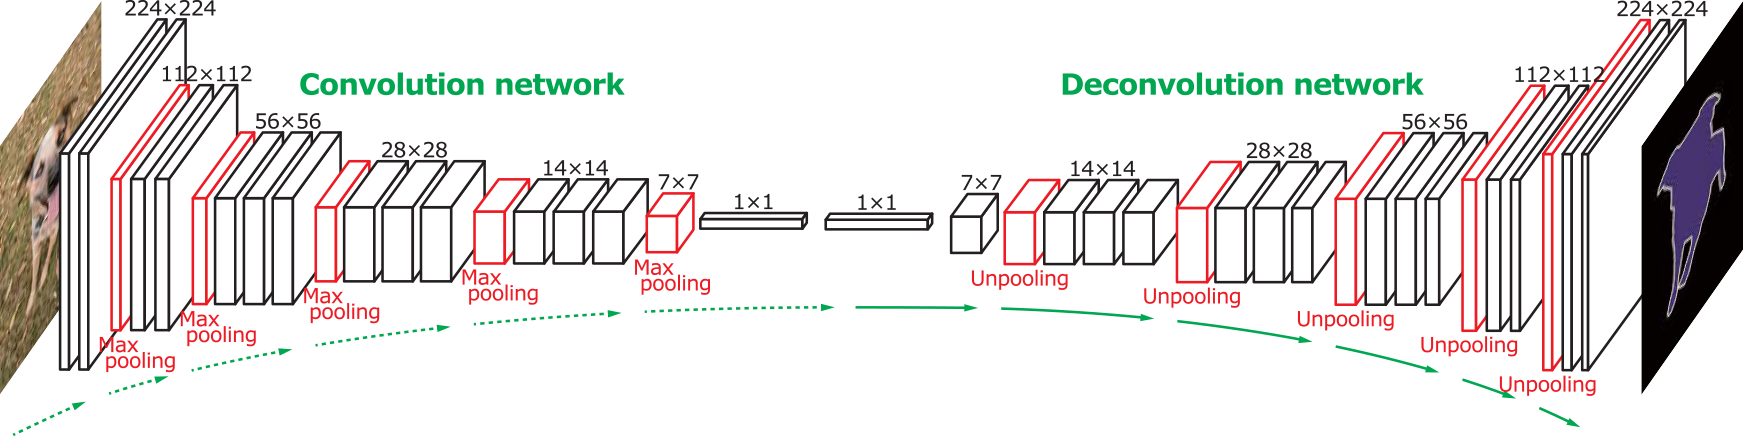
\includegraphics[width=0.9\textwidth]{../images/overall.png}
    \caption*{\scriptsize{Aufbau eines Deconvolution Netzwerkes}}
\end{figure}






\end{frame}